% PREAMBLE
\documentclass[12pt, letterpaper]{article}
\usepackage[utf8]{inputenc}
\usepackage{tipa}
\usepackage[margin=1in]{geometry}
\usepackage[parfill]{parskip}
\usepackage{hyperref}
\usepackage{graphicx}
\title{Pronunciation Checking with ASR\\ \small User Specification}
\author{Evan Nichols}
\date{MFF 2021/2022}

\begin{document}
\maketitle

\section*{What Is It?}
This application allows the user to test their pronunciation of various English sentence prompts. It supports multiple concurrent users. Users record themselves, via the web page, and then wait for their pronunciation to be evaluated. After a short delay, they may pull up their score and review, or try again. It uses a neural network module built for automatic speech recognition to evaluate the speech. The module compares the users' spoken phonemes to those of the text prompt (converted from the text), and compares the differences. The application is built using Flask, a web framework for Python, with a web page run in JavaScript. 

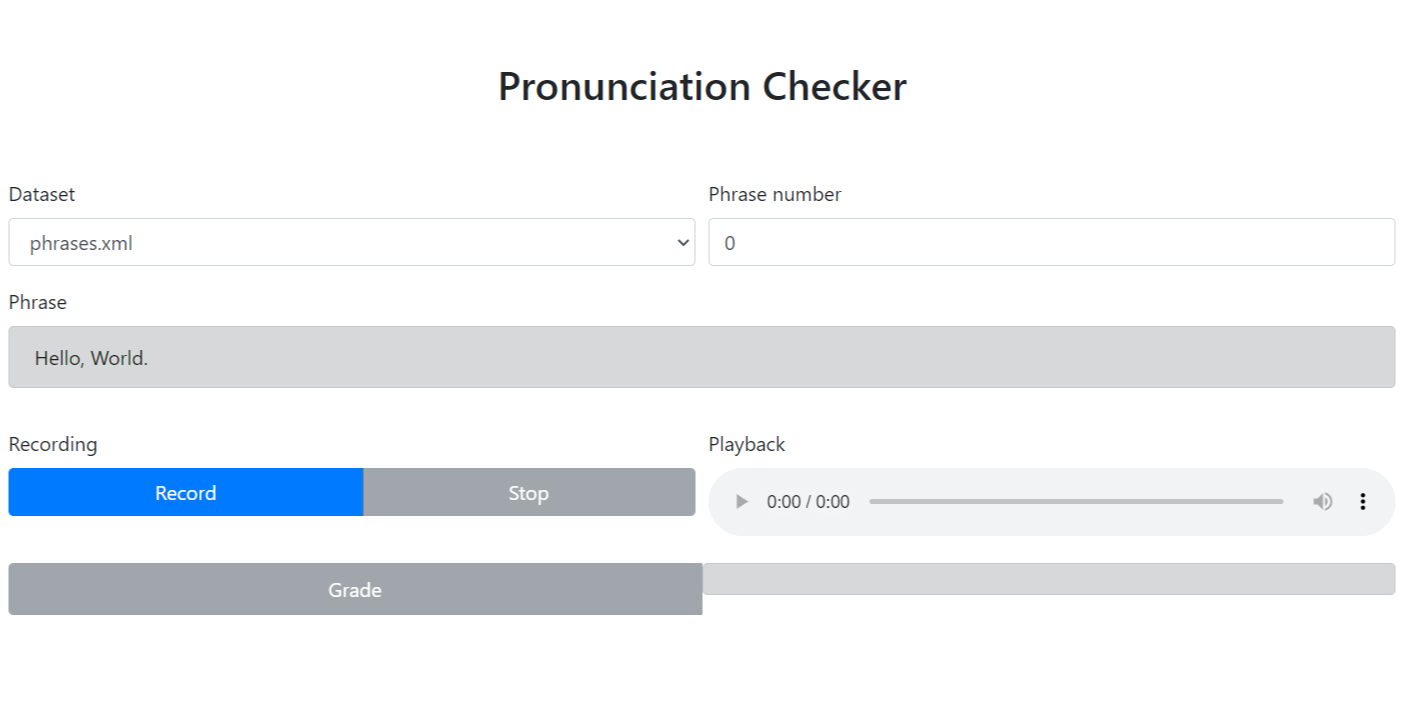
\includegraphics[scale=0.33]{images/homepage.png}


\newpage%######################################################################
\section*{How to Use this Appplication}
Upon loading the web page, the user is presented with a simple interface of a few fields, and will be prompted by most browsers for microphone access. Immediately, the \textbf{Record} button may be pressed. This will begin recording, and the user should read the \textbf{Phrase} text out loud. After speaking the phrase and pressing \textbf{Stop}, the recorded audio is sent to the server-side along with the text prompt and processed and packaged into a data set. This data set is then processed by an automatic speech recognition module and the user's speech audio is graded against the prompt phrase. A score, marking how well the user pronounced the prompt, is stored in a text file and once when the user presses \textbf{Grade} this score is output to them. To add varying challenge, the user may choose from a number of phrases, take from several data sets. 

\subsection*{Phrase Prompts}
The phrases can be any English words and sentences. The prompts do not NEED to be legitimate English, but for the sake of pronouncing words well it makes more sense for them to be actual language. Special characters are irrelevant in the grading, as the program strips items such as '!' and ':' before passing the prompt key to the ASR module. The phrases included in the app as of this writing are taken from various books and poems. 

\subsection*{Input Audio}
The user's speech speech is recorded, the raw data is sent to the back-end and then reformatted to a \textit{.wav} file with a sampling rate of 16000 and 1 audio channel. A \textbf{spectrogram} is also created which displays some information to the user. The spectrogram measures frequency (y-axis) over time (x-axis), and the intensity of the color marks the amplitude of the frequency at that moment.

\begin{figure}[h!]
  \caption{Spectrogram generated for input speech "hello world"}
  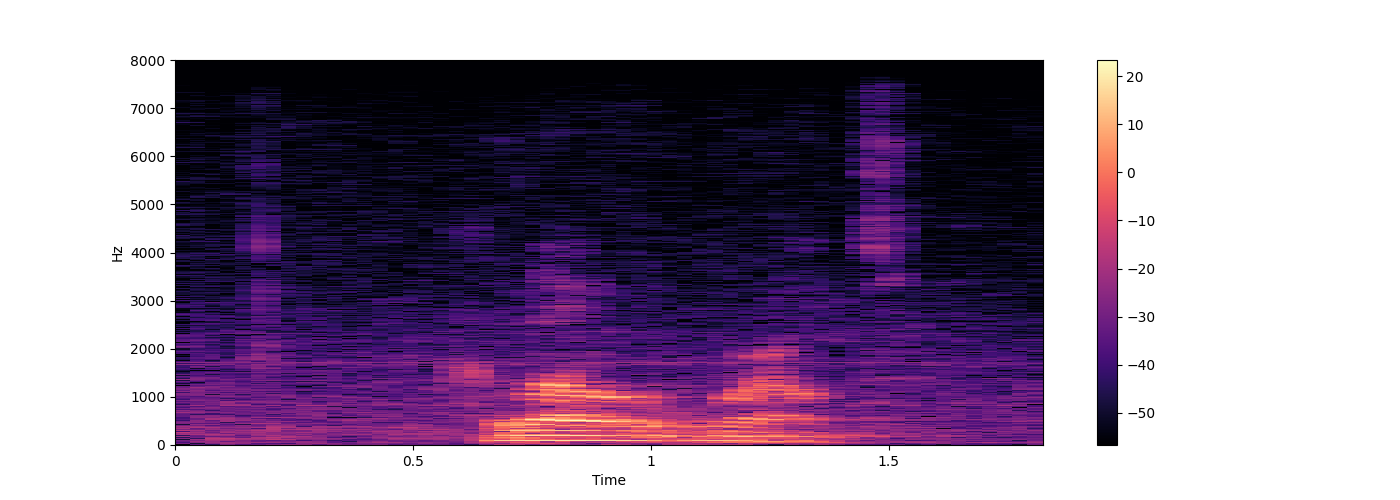
\includegraphics[scale=0.5]{images/sample_spectrogram.png}
\end{figure}

\newpage%######################################################################

\section*{User Interface}


\newpage%######################################################################

\section*{Program Files}
\subsection*{app.js & index.html}
This JavaScript file powers the web page and handles sending requests to the back-end. A \textbf{MediaRecorder} object is used to record and playback the user's speech. Ajax POST requests are sent to \textbf{app.py} with the text prompt and the recorded audio. The program processes this input and feeds back the desired output: the graded speech results, the spectrogram, pronunciation key, and selected phrases. 'index.html' is an HTML layout for the web page with three buttons, an audio playback box, and two selectors for choosing a speech prompt. The user is able to listen to their own recorded audio and to re-record, as well, overwriting any previous input.

\subsection*{app.py}
This is written with Flask, a web application framework. It receives and handles requests from \textbf{app.js}, returns the appropriate responses, and manages the folder '/temp/'. It reformats the input audio using \textbf{ffmpeg}, and turns the text prompt into a pronunciation key with \textbf{Phonemizer}. The spectrogram is generated with \textbf{Librosa}, and several small functions pull phrases for prompts from XML libraries. 

\subsection*{asr.py}
This Python file contains a watchdog loop that waits for any modification to '/temp/\textit{uuid}\_dataset.json' and upon detecting a change it feeds the fresh data set to the ASR module. The module takes the reformatted input audio and phoneme key and evaluates the user's pronunciation, calculating a scored based off the word error rate. The results are stored in '\textit{uuid}\_graded.txt'.

\begin{figure}[h!]
  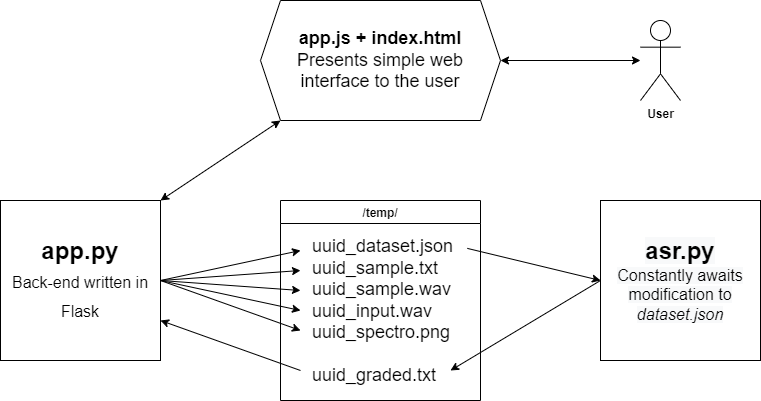
\includegraphics[scale=0.6]{images/workflow.png}
\end{figure}

\end{document}
